Tratemos agora de alguns exemplos pertinentes à teoria desenvolvida. AS figuras aqui utilizadas são resultados das simulações realizadas na seção \ref{sec: simul}.

\subsection{Potencial Gaussiano}

Em geral, para os ensembles gaussianos estaremos interessados no potencial quadrático. Salvo uma escala, se define o potencial

\[
	V(x) = x^2.
\]
Para estes ensembles vale o clássico resultado da medida de equilíbrio dada pela Lei do Semi-Círculo de Wigner. Se expressa,
\[
\supp \mu_V = [-\sqrt{2}, \sqrt{2}], \quad \frac{\dd \mu_V}{\dd x}(x) = \frac{1}{\pi} \sqrt{2 - x^2},
\]
e teremos das simulações para os três ensembles e suas distribuições esperadas na Figura \ref{fig: semicircle}.

\begin{figure}[ht!]
	\centering
	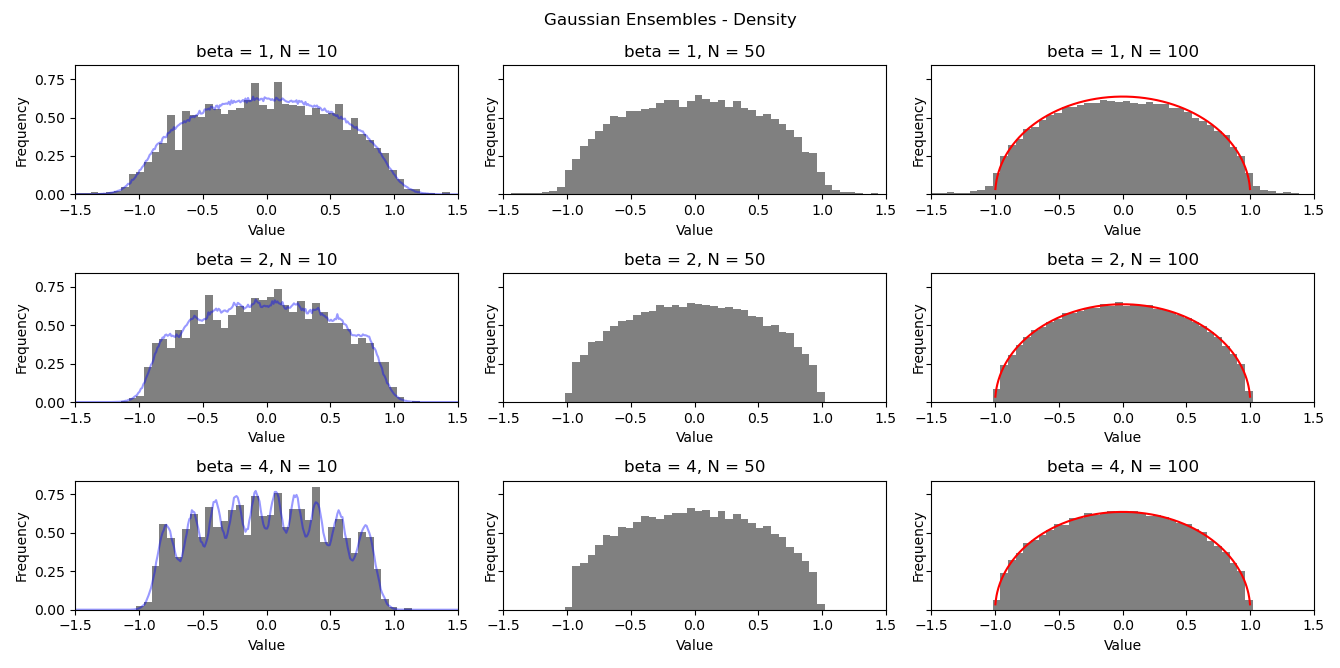
\includegraphics[scale=0.45]{Assets/validationArticleAlg}
	\caption{Validação para ensembles clássicos, utilizamos $200000$ passos registrando a cada $500$ a partir da metade dos passos. $\Delta t = 0.1$, $\gamma = 1$, $\alpha = 1.0$.}
	\label{fig: semicircle}
\end{figure}

Podemos considerar agora outros potenciais. Lembre que isso implica que nossas entradas são correlacionadas, os ensembles de matrizes para este caso não são tão diretos quanto para entradas independentes. Consideraremos para os exemplos $\beta = 2$.

\subsection{Potencial Mônico}

Considere o potencial

\[
	V(x) = \frac{t}{2\alpha} x^{2\alpha},
\]
onde $t > 0$ é escala e $\alpha \in \Z$. A medida de equilíbrio para $\alpha = 1$ é o semi-círculo de Wigner podemos validar na figura com a distribuição em vermelho. Sabemos também que o suporte $[-a, a]$ da densidade é dado por

\[
	a = \left( \frac{t}{2} \prod_{j=1}^{\alpha} \frac{2j-1}{2j} \right)^{-\frac{1}{2\alpha}}.
\]

 Podemos observar os resultados das simulações para este potencial e notar o comportamento obtido e a distribuição teórica em vermelho para o semicírculo em \ref{fig: quarticmonic}.


\subsection{Potencial Quártico}

Considere o potencial

\[
	V(x) = \frac{x^4}{4} + t \frac{x^2}{2}.
\]
Aqui observaremos pela primeira vez uma transição de estado. Teremos um ponto crítico em $t=-2$ onde a medida separa em dois intervalos $[-b_t, -a_t]$ e $[a_t, b_t]$ para $t < -2$ e um único intervalo $[-b_t, b_t]$ para $t > -2$. Ou seja:

\begin{itemize}
	\item \(t > -2\)
	\[
	\supp \mu_V = [-b_t, b_t], \frac{\dd \mu_V}{\dd x}(x) = \frac{1}{2\pi} (x^2 + c_t^2) \sqrt{b_t^2 - x^2} 
	\]
	
	com
	
	\[
		c_t^2 \deff\frac{1}{2} b_t^2 + t \deff \frac{1}{3} (2t + \sqrt{t^2 + 12})
	\]
	
	\item \(t < -2\)
	\[
	\supp \mu_V = [-b_t, -a_t] \cup [a_t, b_t], \frac{\dd \mu_V}{\dd x}(x) = \frac{1}{2\pi} |x| \sqrt{(x^2 - a_t^2)(b_t^2 - x^2)} 
	\]
	
	com
	
	\[
	a_t \deff \sqrt{-2-t}, b_t \deff \sqrt{2-t}
	\]
\end{itemize}

Observamos o comportamento obtido em \ref{fig: quarticmonic}. 

\begin{figure}[ht!]
	\centering
	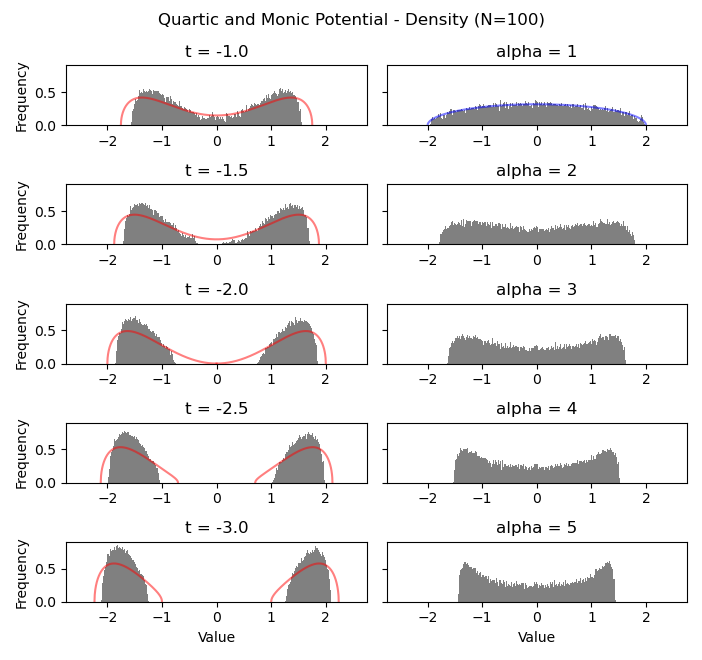
\includegraphics[scale=0.8]{Assets/validationArticleMonicQuarticTheo}
	\caption{Para o potencial quártico, à esquerda, vale $V(x) = \frac{1}{4} x^4 + \frac{t}{2} x^2$. Utilizamos $1000000$ passos registrando a cada $500$ a partir da metade dos passos. Com parâmetros $\Delta t = 0.1$, $\gamma = 10$, $\alpha = 0.1$. Já para o potencial mônico, à direita, vale $V(x) = \frac{t}{2 \alpha} x^{2\alpha}$. Utilizamos $1000000$ passos registrando a cada $500$ a partir da metade dos passos. Com parâmetros $t = 1$, $\Delta t = 0.1$, $\gamma = 10$, $\alpha = 0.1$. Em linha sólida, as distribuições teóricas.}
	\label{fig: quarticmonic}
\end{figure}
